%!TEX root = ../main.tex
The on-vehicle network generally has two types of nodes, a generic sensor node and the wifi node.
This section will seek to design and implement software that adheres to the requirements listed in the table of requirements.
In general all nodes in the system needs to:
\begin{itemize}
\item Get data from CAN network.
\item Send data using a CAN controller.
\end{itemize}
As described earlier, these responsibilities are implemented in the bare-metal CAN program described in section \ref{sec:methods_to_implement_can} therefore these responsibilities will be omitted from the coming sections .

\subsection{Sensor Node}
\label{sec:sensor_node}
The requirements state that it should be simple to add new sensor nodes to the system. 
To realize this the node software should be designed to be modular.
It should be easily identified what software and what interface a developer of a new sensor node must adhere to.

An example of a node can be seen in figure \ref{fig:gps_node}.

%The coming sections will explain the design of the node software that will provide the mentioned functionality using the design requirement.

\begin{figure}[!h]
\centering
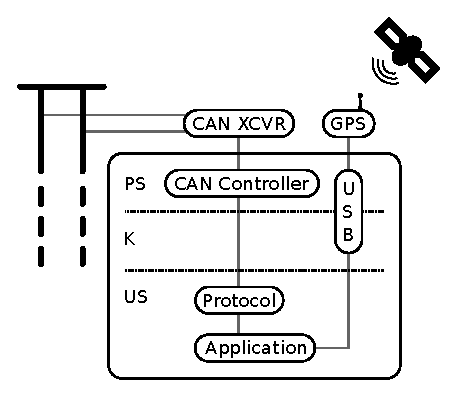
\includegraphics[width=0.5\textwidth]{graphics/analysis_gps.eps}
\caption{GPS node implemented on the Zybo.}
\label{fig:gps_node}
\end{figure}

This specific node has a GPS attached to it connected through a USB interface, but in general it could be any kind of data producing unit connected through any kind of interface.
Due to time constraints, only the GPS sensor software was adapted to function with the designed node software.\\
From the analysis section it is found that a sensor node has the following responsibilities:

\begin{itemize}
\item Get data from associated sensor.
\item Pack data according to the specified protocol.
\item Construct and send CAN package.
\item Receive and execute incoming commands.
\end{itemize}

The three first points describe a flow which is presented in more detail on the flow diagram on figure \ref{fig:filter_1}.

\begin{figure}[!h]
\centering
\begin{subfigure}{0.45\textwidth}
\centering
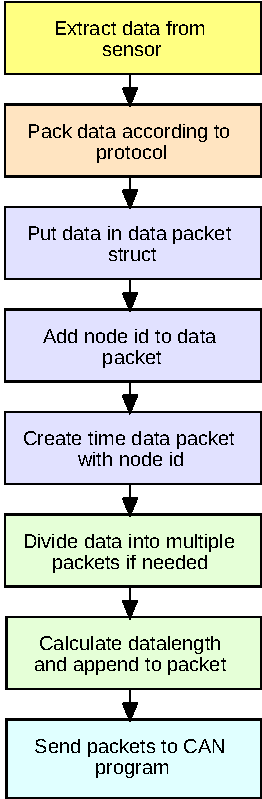
\includegraphics[width=0.60\textwidth]{graphics/FlowChart_Node_Packing}
\caption{Outgoing data. Data from a sensor, to the CAN program.}
\label{fig:filter_1}
\end{subfigure}
~
\begin{subfigure}{0.45\textwidth}
\centering
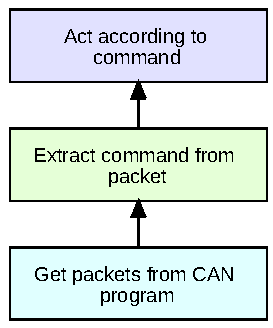
\includegraphics[width=0.60\textwidth]{graphics/FlowChart_Node_Unpacking}
\caption{Incoming data. Data from the CAN program, to the node.}
\label{fig:filter_2}
\end{subfigure}
\caption{Block diagram showing handling of outgoing and incoming data. The boxes are colored according to which class implements the functionality. 
Yellow is the GPS class, orange is the Packer\_GPS class, purple is the node class, green is the protocol class and blue is the CAN\_link class.}
\label{fig:flow_flow}
\end{figure}

It is required to design the software with modularity in mind.
For this, it is necessary to determine which blocks are common for all nodes and which are application specific.
The application specific tasks, in this case, are found to be extracting data from sensor and to pack data according to the protocol.
In principle the task of packing data according to protocol is generic, but the method for packing data depends on data types and messagetypes for the specific application.
The remaining tasks are common for all sensor nodes in the system. 
The procedure when data is going from the CAN program to the node is shown in figure \ref{fig:filter_2}.
In this case, all tasks are found to be common for all sensor nodes.

\subsubsection*{Class diagram}
Based on the previous analysis, a class diagram was developed and can be seen in figure \ref{fig:node_class_diagram}.
The main responsibilities of the classes are shown in figure \ref{fig:flow_flow}.
The classes \texttt{GPS} and \texttt{GPS\_Packer} are application specific and should be developed for each specific application.
In a generic sensor node \texttt{GPS} would be a \texttt{<sensor>} class and \texttt{Packer\_GPS}  would be a \texttt{Packer\_<sensor>}. 
The classes \texttt{CAN\_Link}, \texttt{Protocol} and \texttt{Node} are agnostic with respect to the type of data they receive from the sensor and to the CAN network.
They are generic classes and should be reused when developing new nodes.

\begin{figure}[!h]
\centering
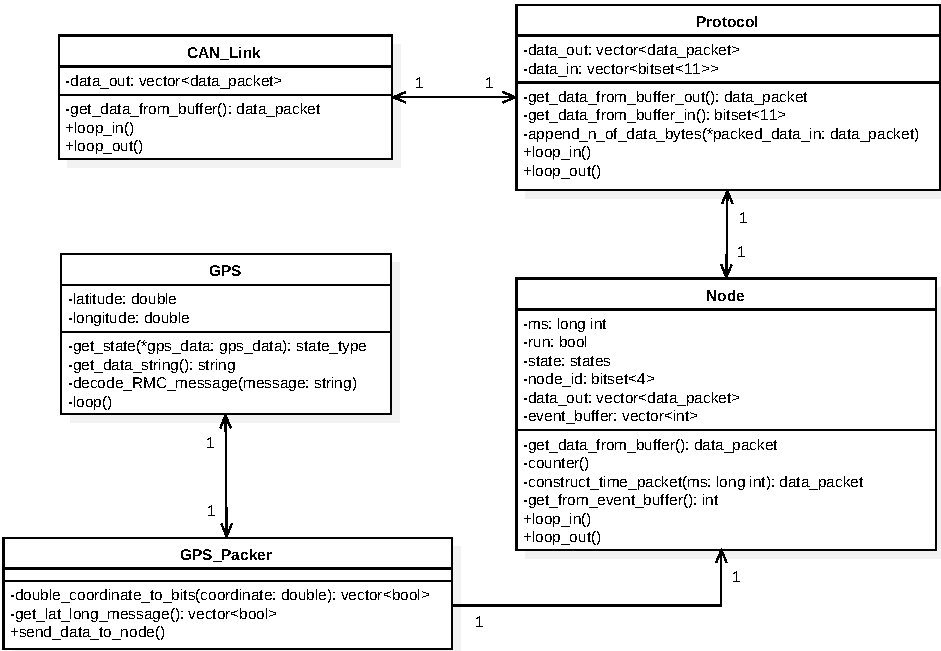
\includegraphics[width=1\textwidth]{graphics/ClassDiagram_NodeSimple}
\caption{Class diagram showing sensor node software.}
\label{fig:node_class_diagram}
\end{figure}

A struct containing all fields of a data packet in boolean data types is defined in listing \ref{code:data_packet}.  

\begin{lstlisting}[caption=Struct for data packet.,label=code:data_packet]
struct data_packet {
  std::bitset<1> nw_msg;
  std::bitset<4> node_id;
  std::bitset<4> dlc;
  std::bitset<6> messagetype;
  std::vector<bool> data; 
  (*@\makebox[\linewidth][c]{$\smash{\vdots}$}@*)
};
\end{lstlisting}
It will be passed between the classes and they will each add their own information. 

The classes and their responsibilities will be explained here in more detail.

~\\ \par \textbf{GPS class} ~ \\
The \texttt{GPS} class needs to extract data from a connected GPS unit and update its own variables with that data.
The specific GPS unit used in this project has a USB interface and uses the NMEA protocol to format data.

~\\ \par \textbf{Packer\_GPS class} ~ \\
The \texttt{Packer\_GPS} class is also sensor specific and is the link between the sensor and the data agnostic node.
It is hard-coded with the message types that the sensor is allowed to send onto the network.
It has the responsibility of packing data according to the developed protocol.
The data field in the \texttt{data\_packet} struct is populated with the GPS data in binary form.
Once packed, the struct is passed to the node class.
The reason for making a separate class for the packer and not putting the functionality into the GPS class is that if the specification of the protocol or message types change, only this class needs to be modified.
Similarly, if the GPS module is replaced, the Packer\_GPS class does not need to be altered.

~\\ \par \textbf{Node class} ~ \\
The Node class receives \texttt{data\_packets} from \texttt{Packer\_GPS}.
Upon receiving a packet, it will set its node ID in \texttt{data\_packet}.
Before sending a message, the associated time packet has to be sent.
In order to create the time packet the class holds a timer which increments each millisecond.
The timer is reset upon receiving a synchronize message.
The class receives start, stop or synchronize events from the protocol class and reacts to those accordingly.

~\\ \par \textbf{Protocol class} ~ \\

The protocol class receives \texttt{data\_packets} from \texttt{Node}. 
If it receives \texttt{data\_} \texttt{packets} with more than eight bytes in the data field, it will split the packet into multiple \texttt{data\_packets}.
The additional \texttt{data\_packets} must have the same node id and message type, but the new message, \texttt{nw\_msg}, bit should be cleared on all but the first message.
The class also needs to count the number of bytes in the data field, \texttt{dlc}, for each \texttt{data\_packet}.
On \texttt{data\_packets} coming from the CAN network the last two bits of the messagetype is used to indicate the type of command sent to the node.

~\\ \par \textbf{CAN\_link class} ~ \\
The \texttt{CAN\_link} class has the responsibility of transferring and receiving data to and from the CAN program.
As this interface has not yet been implemented this class makes use of stdio. 
That is, data from the sensor will be printed in the shell and data to the node is written to the shell. 
\thomas{shell=terminal?}
\subsubsection*{Passing data between classes}
Communication between classes is realised by using the producer-consumer pattern.
As the name implies one class produces data and puts this in a queue where another class consumes by taking data out of the queue.
To get the producer and consumer functions to run in parallel they are run in separate threads.
All queues are protected by mutex to make the software thread-safe.

\subsubsection*{Node class functionality}
The functionalities of \texttt{Node} on outgoing data is implemented using a state machine.
It is shown in figure \ref{fig:state_machine}.
\begin{figure}[!h]
\centering
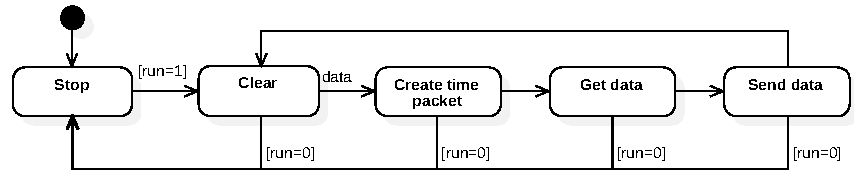
\includegraphics[width=1\textwidth]{graphics/StateDiagram_Node.pdf}
\caption{State machine implementing the functionality of \texttt{Node}. }
\label{fig:state_machine}
\end{figure}
\martin{In figure~\ref{fig:state_machine}, the "boolean" value run, should be the same as the boolean value "running" on figure~\ref{fig:node_class_diagram}.}
When the variable \texttt{run} is equal to 1, the node should output sensor data.
\texttt{run} is being updated by the thread that handles incoming commands.
It will then go the clear state and clear all variables and wait for data. 
When data is present it will move through the states, create the time packet, get data and send data. 
If at any point \texttt{run} is set to 0 the state machine will go to the stop state.
In the stop state the input queue of \texttt{data\_packet} will be cleared.


\subsection{WiFi Node}
The node with a WiFi connection to the stationary computer is a special node in the system.
There should be only one and it should collect all CAN messages, log them and transfer them using WiFi.
Because of time constraints the software designed in this has not been implemented in code.
The WiFi node can be seen in figure \ref{fig:wifi_node}.

\begin{figure}[!h]
\centering
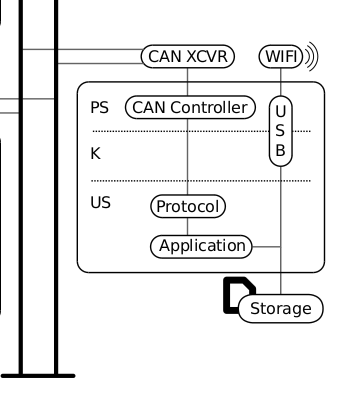
\includegraphics[width=0.4\textwidth]{graphics/wifi_node}
\caption{WiFi node implemented on Zybo board.}
\label{fig:wifi_node}
\end{figure}

From the analysis it is clear that the WiFi node has the following responsibilities:

\begin{itemize}
\item Log all data to SD card.
\item Transmit and receive data through WiFi.
\item Pack data according to protocol.
\item Send log file through WiFi upon request.
\item Timestamp management.
\item Merge multi frame packets.
\end{itemize}
\mikkel{Is multi frame packets what we mean?}
\martin{Yes, I think we mean that.}

It is found that the responsibilities can be grouped into normal operation mode and sending log file mode.
This should be implemented as a state machine as shown in figure \ref{fig:StateDiagram_NodeWiFiStates}.
In normal operation mode the WiFi node should handle data coming from the CAN network and the data coming from the WiFi connection.
If it receives a \texttt{send\_log} command from the stationary computer it should go into the sending log mode and stay there until the log file has been sent.

\begin{figure}[!h]
\centering
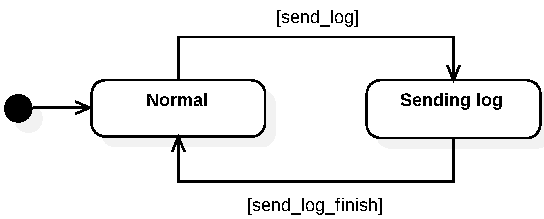
\includegraphics[width=0.5\textwidth]{graphics/StateDiagram_NodeWiFiStates}
\caption{State machine in WiFi node software.}
\label{fig:StateDiagram_NodeWiFiStates}
\end{figure}

In normal operation mode it should handle all incoming data from the WiFi connection as shown in figure \ref{fig:FlowChart_NodeWiFiCmd}.
As it can be seen the WiFi node will only send frames to the CAN network when it receives commands to do so from the stationary computer.

\begin{figure}[!h]
\centering
\begin{subfigure}[b]{0.42\textwidth}
\centering
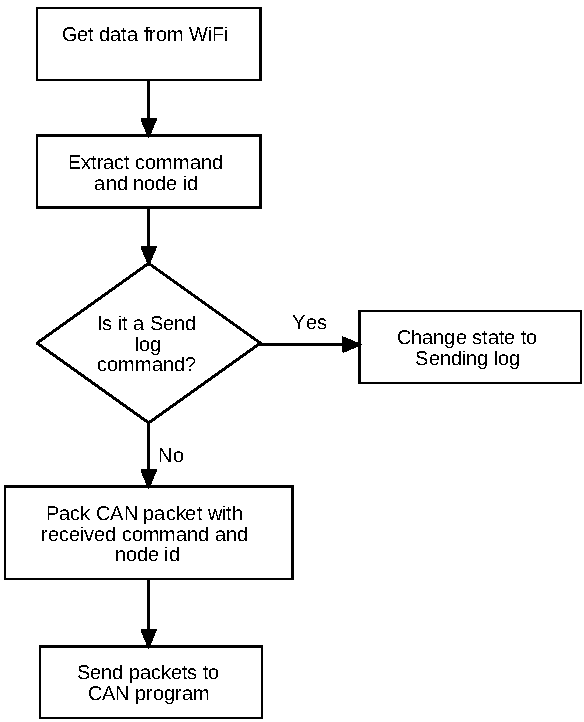
\includegraphics[width=1\textwidth]{graphics/FlowChart_NodeWiFiCmd}
\caption{Handling of data received through WiFi.}
\label{fig:FlowChart_NodeWiFiCmd}
\end{subfigure}
~
\begin{subfigure}[b]{0.52\textwidth}
\centering
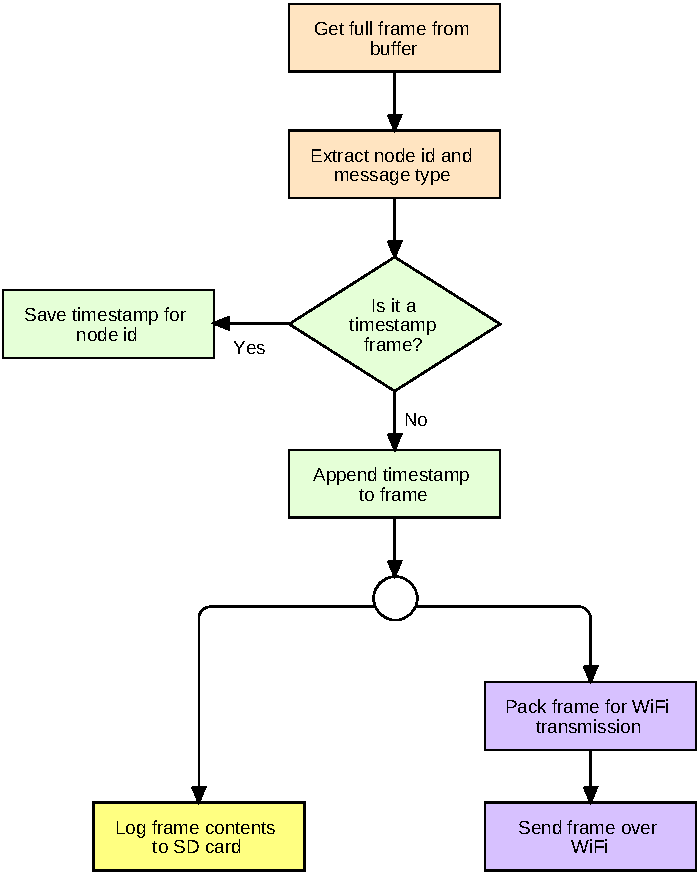
\includegraphics[width=1\textwidth]{graphics/FlowChart_CANFrameProcess}
\caption{Handling of data received from CAN network.}
\label{fig:FlowChart_CANFrameProcess}
\end{subfigure}
\caption{Block diagram showing handling of outgoing and ingoing data. The boxes are colored according to which class implements the functionality. Purple is the WiFi class, pink is the state machine class, orange is the protocol class, green is the CAN\_link class, blue is the timestamper class and yellow is the logger class.}
\label{fig:wifi_flow}
\end{figure}

In normal operation mode the WiFi node needs to receive CAN frames from the CAN program. 
Some frames contain data that is split into multiple frames.
In order to log and timestamp data correctly these frames needs to be merged together.
The \texttt{nw\_msg} field in the messageid will be \texttt{0} if a received frame needs to be merged with the previously received frame.
A state machine handling merging of frames can be seen in figure \ref{fig:StateDiagram_ConcatMsgProcess}.

\begin{figure}[!h]
\centering
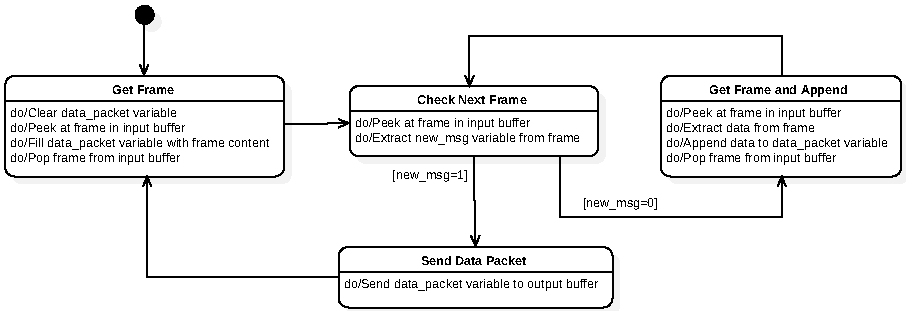
\includegraphics[width=1\textwidth]{graphics/StateDiagram_ConcatMsgProcess}
\caption{Merging multi frame packets together.}
\label{fig:StateDiagram_ConcatMsgProcess}
\end{figure}

The mentioned input buffer is the buffer where the CAN program puts its received frames. 
When the frames are correctly merged they will be put in the merged frame buffer.
The frames in this buffer then needs to be timestamped correctly, logged and sent throug WiFi.
This flow is depicted in figure \ref{fig:FlowChart_CANFrameProcess}.


\subsubsection*{Class diagram}
Based on the previous analysis a class diagram was developed and can be seen in figure \ref{fig:StateDiagram_NodeWiFi}.
The classes main responsibilities are shown in figure \ref{fig:wifi_flow}.

\begin{figure}[!h]
\centering
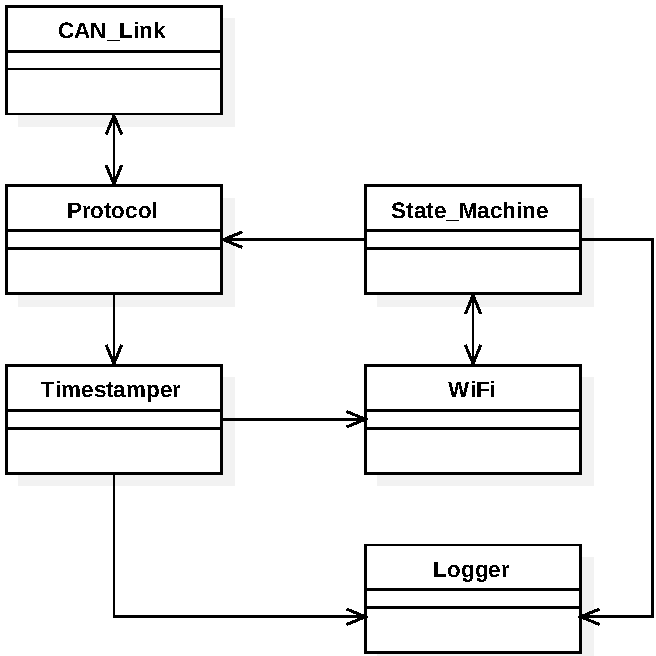
\includegraphics[width=0.6\textwidth]{graphics/ClassDiagram_NodeWiFi}
\caption{Class diagram showing sensor node software.}
\label{fig:StateDiagram_NodeWiFi}
\end{figure}

\mikkel{Should these class descriptions be omitted?}
\subsubsection*{WiFi class}
The WiFi class needs to receive and transmit data through the connected WiFi dongle.
It receives data from the Timestamper class in normal mode and data from State\_Machine in sending log mode.
The State\_Machine also sets if it should transmit the data it gets from the Timestamper class. 

\subsubsection*{State\_Machine class}
The State\_Machine class implements the state machine of figure \ref{fig:StateDiagram_NodeWiFiStates}.
When sending log mode it needs to get a log file from the logger class and give it to the WiFi class.
When i normal mode it needs to extract commands and node IDs from the received WiFi data and give it to the Protocol class.

\subsubsection*{Protocol class}
The Protocol class needs to get frames from the full frame buffer and extract node ID and message type. 
It also needs to pack CAN frames with received commands and node id from the State\_Machine class.

\subsubsection*{CAN\_link class}
The CAN\_link class has the responsibility of transferring and receiving data to
and from the CAN program.

\subsubsection*{Logger class}
The logger class needs to log all received data to a SD-card.
It also needs to read the logged file and transfer it to the State\_Machine classes, when in sending log mode.

\subsubsection*{Timestamper class}
The Timestamper class needs to do the timestamp management described earlier.
It needs to keep the latest received timestamp for each node in the network.
When it receives data from a node it should append the latest received timestamp from that node.  